\section{Principali problematiche di sicurezza}

Combinare una soluzione VPN sicura con una suddivisione della rete interna in compartimenti isolati sarebbe certamente ideale dal punto di vista della sicurezza.
Tuttavia, l'accesso di terze parti alla rete interna di un'organizzazione - siano essi dipendenti, clienti esterni, o altro, aggiunge delle sfide impegnative nel garantire sicurezza.
Ad esempio, se il dispositivo di un dipendente o di un cliente viene compromesso, e questa persona aveva instaurato una connessione VPN con l'azienda, coloro che hanno portato a termine l'attacco possono sfruttare il tunnel VPN come ponte per effettuare attività di ricognizione sulla rete interna dell'azienda, nonostante tutte le misure di sicurezza possibilmente implementate dall'azienda stessa.

Tuttavia, implementando una soluzione VPN moderna, è possibile monitorare il traffico, chi lo ha generato, che tipo di traffico è, e come viene usato. Tenere traccia di queste attività tramite il monitoring delle session riduce i rischi, in quanto permette alle organizzazioni di identificare la sorgente del traffico sospetto e terminarlo se ritenuto opportuno.

\section{Attacchi mirati agli utenti}

Il primo step per ridurre i rischi e proteggere i dati sensibili dell'azienda è assicurarsi che tutti i dipendenti, o chiunque altro sia coinvolto nell'uso delle VPN, sappia che la sicurezza dei dati è una priorità.
Per fare questo, è necessario assicurare un'adeguata formazione a tutti loro, che copra tutti i maggiori pericoli, e le misure di difesa, che potrebbero incontrare.

È indiscutibile il fatto che alla base ci deve essere un'infrastruttura adeguadata e che i dispositivi utilizzati supportino i più elevati standard di sicurezza. Infatti, i conduttori di un potenziale attacco vanno appositamente alla ricerca di, ad esempio, reti WiFI non protette, o cifrature banali da rompere.

\subsection{Furto di credenziali}
Il furto di credenziali è un tipo di crimine che consiste nel trafugare qualcosa che permette alla vittima di certificare la propria identità - ad esempio, email e password.
Una volta rubate le credenziali, colui che le ha rubate avrà gli stessi permessi e gli stessi privilegi della vittima.
Permette al ladro di resettare password, impedire alla vittima di accedere ai suoi stessi account, scaricare dati privati, ottenere accesso agli altri computer nella rete della vittima, distruggere backup, e via dicendo.

Gestire questo tipo di furti, e le loro conseguenze, dovrebbe avere altissima priorità per tutte le aziende, ma anche per i singoli utenti.

Esistono dei servizi, quali https://haveibeenpwned.com, che permettono agli utenti, inserendo il proprio indirizzo email, di verificare se sono stati coinvolti in un data breach - una divulgazione non autorizzata di dati sensibili in seguito ad un attacco ad una azienda. Questi servizi, che lo fanno a fin di bene, ottengono questi dati attraverso il dark web, così come lo fanno dei malintenzionati. Sapere di essere stato coinvolto in un furto di credenziali permette di prevenire un uso scorretto di esse, cambiando la password e aggiungendo misure di sicurezza più efficaci, quali ad esempio una One-Time-Password.

Le credenziali possono essere rubate sotto varie forme: hashes, tokens o anche testo in chiaro. Per trarre in inganno gli utenti, i malintenzionati spesso utilizzano la tecnica del phishing o dello spearphishing. Si tratta di soluzioni economiche ed efficienti, perché si fondando sull'interazione umana, sulla manipolazione e sull'inganno, anziché sullo sfruttamento di vulnerabilità software.

Nel caso di furto di credenziali aziendali, i criminali effettuano una ricognizione per capire chi sono le persone che posseggono i privilegi necessari a raggiungere il loro scopo, e indirizzeranno a loro i tentativi di phishing.

Alcuni modi per prevenire il furto di credenziali sono:
\begin{itemize}
    \item Autenticazione a più fattori
    \item Formazione degli utenti su come riconoscere i tentativi di Phishing
    \item Formazione degli utenti su come impostare password sicurezza
    \item Limitare l'utilizzo delle credenziali aziendali ad applicativi sicuri e controllati
    \item Mantenere aggiornati i sistemi operativi e i software utilizzati
    \item Effettuare regolarmente valutazioni sulle vulnerabilità
    \item Utilizzare strumenti di monitoring del traffico
\end{itemize}

\subsection{Social Engineering}

Social engineering is a manipulation technique that exploits human error to gain private information, access, or valuables. In cybercrime, these “human hacking” scams tend to lure unsuspecting users into exposing data, spreading malware infections, or giving access to restricted systems. Attacks can happen online, in-person, and via other interactions.

Con social engineering si intende quell'insieme di tecniche di manipolazione che vanno a sfruttare l'errore umano per ottenere informazioni riservate, accesso a sistemi protetti o oggetti di valore. Sono particolarmente efficaci contro utenti ingenui e/o ignoranti in materia, che non si aspettano un pericolo. Questo tipo di attacchi può avvenire online, ma anche di persona o al telefono.

\subsubsection{Phishing e Spear Phishing}

Il phishing è un tipo di truffa facente parte delle tecniche di social engineering che è comunemente camuffata in email o sms fraudolenti. La truffa consiste nel far raggiungere alla vittima la pagina di login di un sito web, dall'aspetto identica a quella del servizio di cui si vogliono rubare le credenziali, che però, anziché portare correttamente a termine il login, inoltra le credenziali al truffatore.
Tra le informazioni nel mirino dei truffatori si ha:
\begin{itemize}
    \item Username
    \item Password
    \item Indirizzo Email
    \item Residenza
    \item Numeri di carte di credito
    \item Data di nascita
\end{itemize}

Lo Spear Phishing è un caso particolare di phishing in cui il malintenzionato ha studiato la vittima e le sue abitudini. Per aumentare le possibilità di successo, infatti, includerà nel messaggio fraudolento quante più informazioni personalizzate possibili in modo da far abbassare la guardia della vittima.

Nonostante alcuni tentativi di phishing siano effettivamente ben costruiti, la maggior parte è facilmente riconoscibile.

Di seguito, alcune bandiere rosse per identificare un messaggio fraudolento:

\begin{itemize}
    \item errori ortigrafici e grammaticali: ad esempio, è difficile che una banca invii un messaggio non curato
    \item messaggi contenenti richieste di infromazioni personali: ad esempio richieste di credenziali per accedere a un servizio
    \item messaggi estremamente orgenti: ad esempio, un messaggio inaspettato contenente una minaccia di chiudere l'account della vittima
    \item email contenenti mittenti sospetti: ad esempio, una email proveniente da john@mybankofamerica.com, quando il dominio usuale è @bankofamerica.com
\end{itemize}

\section{Attacchi mirati al sistema}
\subsection{Versione non aggiornata}
\subsection{Exploit di vulnerabilità zero-day}

\section{Multi-factor authentication}
Among the main reasons you should ensure additional VPN security is the trend of phishing attacks, which are successfully performed by criminals in up to 17\% of cases, according to the Duo report.
Phishing is a  social engineering technique when a hacker contacts a person either via email, SMS, or a phone call, pretends to be a reputable organization representative, and persuades their victim to provide their credentials. Often the phishing email or message may contain an attachment with malware or a link that leads to the fake website, anyway, the main goal of the hacker, who performs the phishing attack is to get the user credentials.
If the phishing attack is successful, the hacker may get the login and password required to connect to the corporate system through the VPN. Then, the hacker would be able to enter this user's profile, and install the malware, or steal sensitive data from the server computer.
An extra layer of authentication guarantees that the network cannot be breached by outside players, even if they possess the stolen credentials. VPN two-factor authentication verifies the identity of the user not only by a single password but by a time-based one-time password. It is much harder to steal and use such a one-time password as it's valid only for 30 seconds, thus guarding against phishing and other security threats (brute force, keyloggers, MITM attacks, etc).

\begin{figure}[ht]
    \centering
    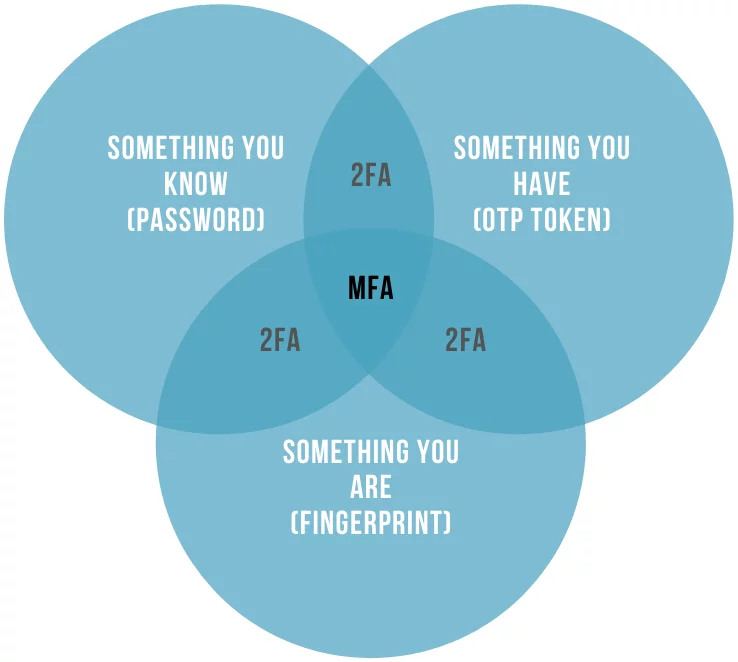
\includegraphics[width=12cm]{figure/mfa.jpeg}
    \caption{MFA}
\end{figure}

\subsubsection{Certificato}
Certificates can be used for authenticating VPN gateways and the Stonesoft VPN Client.

In site-to-site VPNs, you can use both pre-shared keys and certificates as the authentication method. In mobile VPNs, certificates are always needed when the Stonesoft VPN Client is involved. However, if you use the hybrid authentication method with the Stonesoft VPN Client, only the gateway needs a certificate.

What VPN certificates do

Certificates do not contain information that is specific to a particular VPN. You can use certificates for authentication in both the policy-based and route-based VPNs. A certificate authority (CA) issues certificates as proof of identity. Gateways that form a VPN tunnel are configured to trust the CA that signed the other gateway's certificate. All certificates issued by a trusted CA are accepted as valid, so certificates can be added, renewed, and changed without affecting the VPN as long as the actual identity information is correct. The same certificate can be used for any number of VPNs with any number of gateways and VPN clients.

Certificates are always required for gateways to which the Stonesoft VPN Client connects. Certificates can optionally be used to identify VPN clients, but are not mandatory.

Certificates reduce the required maintenance work, because they do not have to be changed as frequently as pre-shared keys. All certificates are created with an expiration date, after which the certificate is no longer valid. Certificates signed by an Internal RSA CA for Gateways or an Internal ECDSA CA for Gateways are valid for three years from their creation. When a certificate expires, a new certificate is needed.

Certificate management

Certificate-related tasks in the SMC mostly involve VPN Gateways that represent firewalls. VPN certificates can be generated by any internal or external certificate authorities that both gateways are configured to trust. There are several options for signing VPN Gateway certificates:

The Management Server includes a dedicated Internal RSA CA for Gateways and optionally an Internal ECDSA CA for Gateways for signing VPN certificates. You use these certificate authorities through the Management Client.
One Internal CA for Gateways can be selected as the default CA. Certificate management can be automatic if the certificate is signed using the Management Server's internal default CA.
You can create certificate requests in the Management Client, export them, sign them using an external CA, and then import the signed certificate back into the SMC.
RSA certificates can be created and renewed automatically using the default CA. Some manual steps are required in the following cases:

You have both an Internal RSA CA for Gateways and an Internal ECDSA CA for Gateways. Only one Internal CA for Gateways can be selected as the default certificate authority. You must manually create and renew any certificates that are not signed by the default CA.
You use DSA certificates.
You want to use an external CA to sign certificates.
The Internal RSA CA for Gateways or Internal ECDSA CA for Gateways can also sign certificate requests created by external components. This feature is meant to support VPN client deployments. If you have used the Internal RSA CA for Gateways or Internal ECDSA CA for Gateways to sign certificate requests, you cannot cancel the issued certificates. Consider how widely you can use them for signing external certificate requests within your organization.

Limitations

All gateways in the same VPN must support the same CA algorithm. Otherwise, VPN communication fails. For example, if you use an Internal ECDSA CA for Gateways as the default CA, all other gateways used in the same VPN must support ECDSA.
Certificates created for VPN gateways for establishing the VPN are stored on the VPN gateway devices (Firewalls). These certificates are not included in the Management Server backup, and are not changed in any way when a Management Server backup is restored.
Certificates can become unusable if the private key for that certificate is lost. The key can be lost, for example, if the NGFW Engine hardware fails and must be replaced. Firewall Clusters share each VPN certificate and can synchronize the private key from node-to-node as needed. If the private key is erased from a Single Firewall or from all the nodes of a Firewall Cluster, a new certificate must be created.
Externally issued VPN certificates can be revoked by the certificate authority that issued them. This safety measure is used when the certificate is suspected to be compromised.

\subsubsection{Username e password}
Password authentication is the easiest way to use for identifying and authenticating users. A password is established for the user if using password authentication.
Users will be refused to be accessed, if the password doesn't match when they attempt to connect to VPN. Users can change the password registered in VPN Server themselves at any time using VPN Client. For details see 4.9 Other Functions.
The passwords for password authentication are registered in the configuration database of SoftEther VPN Server. At this time the password is hashed by hash function, so the original password no longer exists. When conducting password authentication, SoftEther VPN protocol checks passwords for user authentication by challenge and response authentication (digest authentication). At this time the original password is not transmitted on the network.
The drawbacks of password authentication are as follows.
If there are few users, operation can be conducted with no problem, but if there are more than several hundred users, it takes effort to register/delete users. In such cases, RADIUS authentication, NT domain or Active Directory authentication is used.
The password base authentication method is connected with weaknesses such as the possibility of the password being guessed. Certificate authentication is used if corporate security policy does not recommend the password base authentication method and higher security is required.


\subsubsection{One Time Password}
Two-factor authentication (2FA) prevents hackers from having access to your network using compromised credentials. 2FA calls for customers to validate their identification by supplying a 2nd safety component in addition to their password. When connecting to a company network, users have to first input their Active Directory credentials, followed by a time-factor based one-time password (OTP) or HMAC. This OTP is displayed on something that a user “owns”, including a specialized cell phone application known as an authenticator or a programmable hardware token. Ultimately, this provides an additional layer of security for your systems against unauthorized access.

2FA with mobile token

How VPN security is achieved with 2FA?
VPNs are a vital part of many businesses' security infrastructures, providing employees with secure remote access to company resources. However, VPNs can also be vulnerable to attack if they are not properly secured.One way to help secure a VPN is to use Two-Factor Authentication (2FA) for all users. 2FA requires users to provide more than one form of authentication to access a system or resource. For example, a user might need to enter a password and also use a fingerprint reader or mobile device for two-factor authentication.2FA can be used to help secure both the client-side and server-side of a VPN connection. On the client side, 2FA can be used to authenticate the user before the VPN client software is even launched. This helps prevent attackers from launching the VPN client software with stolen credentials.On the server side, 2FA can be used to authenticate VPN users when they attempt to connect to the server. This helps ensure that only authorized users are able to access the server and helps prevent man-in-the-middle attacks. 2FA is not a perfect solution, but it can be an effective way for your VPN security.

One-time tokens are typically generated with an authentication app such as Google Authenticator, or a piece of hardware with a small display. These apps cycle through six-digit tokens, which the user reads and then enters along with the password when logging in, for example “123456mypassword”.

Because the password is transmitted via PAP, the RADIUS server can see the entire password field and can split the value “123456mypassword” into two parts. The token part: “123456” is verified against the OTP token server. The password part “mypassword” is verified against the user directory such as LDAP or Active Directory in the usual way. If either check fails, the user is rejected. If both checks pass, the user is authenticated.



